\chapter{Summary of contributions}\label{ch:content}
The following is a summary of the main contributions in this thesis.
All presented approaches deal with dataset bias that is closely linked to a special attribute $s$.
In terms of \citet{kamishima2012fairness}'s taxonomy (see section \secref{fair-classifiers}),
this can be described as tackling \emph{negative legacy} that is mediated by \emph{prejudice}.
Furthermore, the approaches all rely on some form of side information which allows us to overcome dataset bias.
This side information is always significantly easier to obtain than unbiased data.

% - suddenly images?
% - (explain in the linking chapter)
% - is it specific to images?
% - explain how it works for tabular data

\section{Mitigating label bias with target labels}\label{sec:target-labels}
The first work is \citet{kehrenberg2020tuning} (\chapref{ch:paper1})
which is predominantly concerned with label bias.
More precisely, labels \(y\) are flipped with a probability and a direction that depends on a sensitive attribute \(s\).
The main idea is that we make use of pseudo labels (or \emph{target labels})
to implicitly learn from a \emph{balanced} dataset,
in which \(y\perp s\) holds, and which thus satisfies \acf{DP}.
This falls under the area of \emph{fair classifiers} discussed in \secref{fair-classifiers}

\begin{figure}[tp]
  \centering
  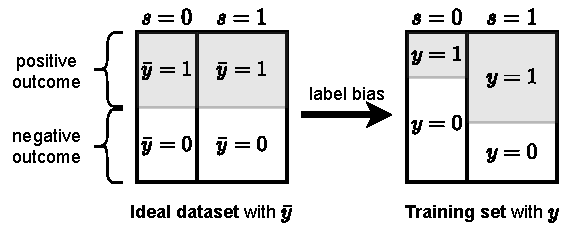
\includegraphics[width=0.9\textwidth]{figures/label_bias.pdf}
  \caption{%
    A diagram of a simple case of label bias, where both the class label \(y\) and the sensitive attribute \(s\) are binary.
    On the left, we have the ideal (possibly fictional) dataset with the target labels \(\bar{y}\),
    where the proportion of positive outcomes is the same for both demographic groups;
    and on the right, the training labels, for which the proportions are \emph{not} the same.
  }%
  \label{fig:label-bias-overview}
\end{figure}

We can interpret the contributions of this publication in two ways.
The first corresponds to the definition-centric view of dataset bias,
and the second to the ground-truth-centric view.
\begin{enumerate}
  \item
    We can say that the classifier should satisfy demographic parity in its predictions,
    and learning from a balanced training set is just one particular way to achieve this.
    In this view, the pseudo labels have no deeper meaning and are just a computational trick.
  \item
    We can see the training set as a corrupted version of a true dataset, which is balanced (\(y\perp s\)),
    and so, by learning from these pseudo labels, we are simply approximating the true dataset.
    However, we do not actually have access to the true dataset; we only know that it is balanced.
    In order to evaluate the trained model, we compute fairness metrics with respect to \ac{DP}.
\end{enumerate}
Within the paper, we sometimes jump between these two views.

While the main focus is on label bias,
the experiments are performed on real-world fairness datasets,
which also display a significant amount of sample bias (disadvantaged groups are underrepresented).
Furthermore, in addition to the result for \ac{DP}, we also show that the proposed scheme improves \acf{EOpp}.

In order to construct the target labels,
we use side information about summary statistics for a balanced training set.
This allows us to target a specific balanced set, instead of just any balanced set.
In other words, rather than just enforcing \ac{DP}, the method gives control over the target rates \(P(\hat{y}=1|s)\),
which are the only fairness-hyperparameters of the model.
The target labels \(\bar{y}\) represent an uncertain estimate of labels corresponding to a balanced dataset
(one where \(\bar{y} \perp s\); see also \figref{fig:label-bias-overview}).
The idea is then the learn a predictor for these target labels instead of the given (biased) training labels \(y\).
Via the sum rule of probabilities, it is possible to express the model likelihood in terms of the target labels,
such that maximising the likelihood corresponds to improving the prediction of the target labels.

The requirements for the model are that it outputs probabilities
and that they are well-calibrated --
which means that for those samples
that the model predicts a 10\% chance of having a positive label (\(y=1\))
about 10\% in fact have a positive label,
and analogously for all other predicted probabilities.
The probabilities are needed for calculating the expected target label,
and the calibration ensures that this expectation is sensible.
Thus, we picked a \acf{GP} model as one model for the experiments,
as they have a reputation for being well-calibrated.
However, they come with the downside that they are (at least in their standard form)
not well-suited to very high dimensional data like images.
As such, we also construct a model based on \acf{LR}.

The method is validated with experiments
on the UCI Adult Income dataset and the ProPublica/COMPAS dataset,
which have been mentioned several times in \chapref{ch:related-work},
and which are the most common tabular fairness datasets.
While both these datasets comprise only tabular data,
there is nothing in principle that stops this method from being used for other kinds of data.
The choice to use these datasets and not others
was predominantly made for easier comparison to baselines,
and shorter experiment runtime.

\section{Overcoming severe sampling bias with a representative set}\label{sec:nifr}
In the setting from the above paper \citep{kehrenberg2020tuning},
labels were untrustworthy because they had been flipped;
a phenomenon we referred to as \emph{label bias}.
However, flipping labels is not the only way that labels can become untrustworthy.
Another way is \emph{sampling bias}, which is the subject of \citet{kehrenberg2020nullsampling} and \citet{kehrenberg2020zeroshot} (\twochaprefs{ch:paper2}{ch:paper3}).

As an example, consider the scenario where someone wants to create a classifier
to distinguish between sheep and cows, that is supposed to work anywhere on earth.
However, they take a shortcut while creating the dataset
and take all their sheep images from hot and dry countries
and all their cow images from mild and rainy countries.
In this case, the dataset is lacking cow images in dry landscapes,
and is lacking sheep from green landscapes;
the dataset exhibits a strong sampling bias.
The result is that even though the labels correctly correspond to cows and sheep,
they do not point reliably to the right target anymore.
As background colour is easier to recognise with a \ac{CNN} than animal species,
the labels have effectively been turned into landscape labels.
In other words, landscape has become a \emph{spurious attribute}.
%
% As an example, consider a dataset where the task is to distinguish smiling from non-smiling faces.
% Say, we initially have a very diverse and balanced training set,
% but then, from the set of smiling faces, we remove nearly all samples where the person does not have red hair,
% and from the set of non-smiling faces, we remove nearly all samples with non-black hair.
% The result is that even though the labels are still correct, they do not point reliably to the right target anymore.
% As hair colour is easier to recognise with a \ac{CNN}, the labels have effectively been turned into hair colour labels.
% In other words, hair colour has become a \emph{spurious attribute}.
In the following, we denote the spurious attribute with \(s\),
as it takes on a role that is very similar to that of the sensitive attribute that was also denoted by \(s\).
However, there is a difference in emphasis between a \emph{sensitive} and a \emph{spurious} attribute:
the former indicates that the attribute should not be used for legal or ethical reasons,
whereas the latter can be any attribute that is associated with the class label \(y\) in an undesired way
that leads to lower quality generalisation.

The method, proposed in the previous paper (\chapref{ch:paper1}),
is not able to deal with such a dataset bias as we can easily see:
Say, \emph{smiling} corresponds to \(y=1\) and \emph{not smiling} to \(y=0\);
furthermore, let red hair correspond to \(s=1\), black hair to \(s=0\), and all other hair colours to \(s=2\).
Then, the problem with the described dataset is, that it mostly consists of samples with \(y=0\wedge s=0\)
and those with \(y=1\wedge s=1\).
If we call \(P(y=1|s=s')\) the acceptance rate,
then the problem can be described as one of very different acceptance rates in the hair colour groups given by \(s\).
This is the problem tackled in the previous paper,
and yet, if we were to equalise the acceptance rates with the method there,
the result would be very incorrect.
The issue is that we would treat the labels as incorrect, when in truth, they are correct;
the problem with the data being sampling bias.

To deal with sampling bias, a different approach is needed.
Indeed, the problem, as posed, is not solvable in the general case.
To make headway with this problem, we introduce the concept of a \emph{representative set}.
This set is not subject to the sampling bias,
but is unlabelled (with respect to $y$) and so does not by itself suffice for training.
However, this set does have labels for the spurious attribute \(s\).
This allows us to learn an \emph{invariant representation},
\ie, a representation of the input features \(x\) which is invariant to the spurious attribute.
This kind of representation is equivalent to a fair representation -- as described in \secref{sec:fair-representation} --
which is invariant to a sensitive attribute.
With the invariant representation of the training set,
a classifier can then be trained to accurately predict the class label \(y\).
The invariant representation cannot be learned from the training set
because there, due to the sampling bias, \(s\) and \(y\) are not sufficiently distinguishable.

A parallel to the previous paper is that the method makes use of side information
(in this case the representative set)
in order to overcome the bias in the training set.

The method implementing this general strategy, and presented in \citet{kehrenberg2020nullsampling} (\chapref{ch:paper2}),
is based on the idea of \emph{null-sampling},
which refers to zeroing out part of an encoding,
and then reconstructing the modified encoding as if it were a normal encoding.
In order to apply null-sampling, an encoding of the input \(x\) is learned that is split into two parts:
\(z_u\), which has no information about the spurious attribute \(s\),
and \(z_b\), which has all the remaining information needed to reconstruct \(x\) that is not contained in \(z_u\).
\(z_u\) is ensured to be not predictive of \(s\) via adversarial training.
During null-sampling, \(z_b\) is zeroed out, and after decoding it,
we obtain an invariant representation \emph{in the data domain}.
The fact that it is in the data domain makes it interpretable (or inspectable)
as defined in \chapref{ch:introduction}.

The described method works particularly well with \acp{INN},
as they ensure that no information is lost that is unrelated to \(s\).
However, the price to pay for using \acp{INN} is higher memory requirement and slower training.
Thus, we also present a variant of the method using \iac{VAE},
which does not have the guarantee about preserving information,
but also does not suffer from the increased training cost as much.
\acp{VAE} are similar to \acp{INN}
in that their encoding conforms to a specific probability distribution,
from which we can sample our null-samples.
The choice between the two presented variants is determined
by whether the user is willing to accept higher training costs
for a lower probability of losing information needed for any prediction tasks.
However, the key element is simply any kind of encoder -- producing a split-encoding --
whose output can be subjected to adversarial training,
so encoders other than \acp{VAE} or \acp{INN} will potentially work as well.

We perform experiments on the Coloured MNIST dataset (as described in \secref{sec:groundtruth-centric-view-of-bias}),
which has a one-to-one mapping between the class label (\ie, digit) and the spurious attribute (colour)
in the training set.
As colour is ``easier'' to learn, a neural network will learn to predict \(s\) instead of \(y\).
For additional experiments on the CelebA dataset (another image dataset)
and the UCI Adult Income dataset (a tabular dataset),
we deliberately apply sampling bias to the training set and then apply our method.
For the tabular dataset, an autoencoder is trained to produce a continuous representation,
which is then fed into the \ac{INN} or \ac{VAE} model.
Thus, we demonstrate that the method is \emph{general}
in the sense that it is applicable to both image-based and tabular datasets
and furthermore should be applicable to other modalities as well.
For the main experiments, we focus on image datasets,
because they are easiest to visualise in a document.

\section{Overcoming sampling bias with an unlabelled deployment set}\label{sec:zsf}
A shortcoming of the approach from the previous publication \citep{kehrenberg2020nullsampling}
is its reliance on a representative set which has labels for the spurious attribute \(s\).
As discussed, it is necessary to make use of \emph{some} kind of side information,
but perhaps we can relax some requirements.
In particular, while it is already easier to collect data without \(y\) labels (but with \(s\) labels),
it is even easier to collect data without \emph{any} label.
Thus, requiring only an unlabelled context set would improve the applicability of the method.
\citet{kehrenberg2020zeroshot} (\chapref{ch:paper3}) presents an approach based on that idea.

The setting is very similar to the previous publication \citep{kehrenberg2020nullsampling}:
the training set suffers from severe sampling bias, but we have access to a (mostly) unbiased \emph{deployment set}
(similar to but not quite identical to the previously discussed \emph{representative set}).
The idea is that the deployment set corresponds to the setting in which the model is meant to be deployed.
The change from the previous setting is that this additional set may be completely unlabelled,
but in exchange, we have some stronger requirements for the training set:
The holes left by the sampling bias may not be so numerous
as to make \(s\) and \(y\) completely indistinguishable.
For example, in the previous work, the example of Coloured MNIST had a training set
where there was a strict one-to-one mapping of colour and digit;
but this kind of blending of \(s\) and \(y\) into one is not the focus of this paper.
Instead, the focus is on a setting where the training set lacks certain combinations of \(s\) and \(y\),
which results in poor predictions for these combinations on the test set (or deployment setting)
where those combinations \emph{do} occur.
We refer to these missing combinations as \emph{subgroup bias} or \emph{missing subgroups},
depending on whether a given \(s\) value appears in the training set at all.
The label \(s\) plays here a similar role to the spurious attribute in the previous publication,
but as there is a change in emphasis, we refer to \(s\) as \emph{subgroup label}%
\footnote{This terminology is inspired by the \emph{subclass} concept in \citet{SohDunAngGuetal20}.}
instead.
The difference between a spurious attribute and a subgroup label is that
the former is mostly characterised via its confusion with the prediction target,
whereas the latter refers to natural groups in the data
which have differing levels of annotation quality which affects the classification performance on these subgroups.
However, in both cases, the goal is to make the model output invariant to the \(s\) label,
\ie the classification performance should be independent of the subgroup.

As in the previous paper, the first step is to train a neural network to produce an invariant representation.
The second step is then to train a classifier on said representation.
The invariant representation is trained by performing \emph{distribution matching} between the training set and the deployment set.
% Finally, the training set is transformed into the invariant representation,
% to serve as training set for the classifier.

The distribution matching is realised with adversarial networks which compare batches of samples,
in order to try to distinguish data drawn from the training set and the deployment set.
This process requires balanced batches as an inductive bias,
because the network will only learn the intended difference between training and deployment set,
if the drawn batches exhibit this difference.
For example, if batches drawn from Coloured MNIST differ not in colour but in digit class,
then distribution matching will learn to change digit shapes.
Balancing batches from the training set is easily possible with the available labels,
but those are not available for the deployment set,
so we use clustering techniques to identify the different groups in the deployment set,
and then draw samples for the batches at an equal rate from all clusters.
It is important to note here that imperfections in the clustering are not a problem
as long as the batches show on average the intended difference between training and deployment set.

The absolutely essential elements for this method are the encoder (also referred to as `de-biaser')
that encodes both, samples from the training set and samples from the deployment set,
to a splittable representation;
the adversary that tries to identify, from one part of the split representation,
which dataset the given samples originated from;
and some kind of reconstruction loss
to ensure the splittable representation represents the input data well.
The following elements are in theory optional,
but are needed for the method to work with real-world data:
clustering and sampling to ensure that the training batches are balanced in specific ways;
subdivision of the batches into bags; and the aggregation of the adversarial loss over the bags.
Roughly speaking, these elements strengthen the supervision signal for the invariance learning.

Experiments are performed on the same datasets as in the previous papers:
Coloured MNIST, UCI Adult Income and CelebA.
Again, these datasets were chosen, because image data is easy to visualise,
and because demonstrating the method on tabular data provides evidence for the generality.

% \section{Claims and contributions}%
\section{List of publications and author contributions}%
\label{sec:claims-contributions}
This thesis is based on 3 publications (one of which is a work in progress),
corresponding to \rangechapref{ch:paper1}{ch:paper3}.
% The first one is concerned with \emph{label bias} and the other two with \emph{sampling bias}.
The following is a detailed listing of all the individual author contributions.

\subsection{Publication 1}
\begin{refsection}[allreferences]
    \nocite{kehrenberg2020tuning}
    \printbibliography[heading=none]
\end{refsection}
\noindent A shorter version was published as a workshop paper:
\begin{refsection}[allreferences]
    \nocite{kehrenberg2018interpretable}
    \printbibliography[heading=none]
\end{refsection}
\noindent\textsc{Contributions:}
\begin{itemize}
  \item I conceived the idea of using Target Labels to target a balanced set.
    I developed the proof from a starting point that my supervisor pointed me to.
    I wrote all of the code dealing with the modified loss function and nearly all of the remaining code as well.
    I ran most of the experiments and wrote all of the methods section and most of the remaining text as well.
  \item Z. Chen was a discussion partner and helped run the experiments, and wrote some parts of the code.
  \item N. Quadrianto suggested the initial direction of the work, was a discussion partner,
    and helped write the introduction and related work.
\end{itemize}

\subsection{Publication 2}
\begin{refsection}[allreferences]
    \nocite{kehrenberg2020nullsampling}
    \printbibliography[heading=none]
\end{refsection}%
\noindent\textsc{Contributions:}
\begin{itemize}
  \item I conceived the idea of using an \acf{INN} and a representative set to learn an invariant representation.
    I wrote a large part of the code, and ran about half the experiments. I wrote a significant part of the text.
  \item M. Bartlett developed a large part of the tricks needed for training the \ac{INN} successfully.
    He wrote a significant part of the code, and of the text.
  \item O. Thomas helped with writing the code and with running the experiments.
  \item N. Quadrianto gave feedback on the progress and suggested directions to explore.
\end{itemize}

\subsection{Publication 3 (work in progress)}
\begin{refsection}[allreferences]
    \nocite{kehrenberg2020zeroshot}
    \printbibliography[heading=none]
\end{refsection}%
\noindent\textsc{Contributions:}
\begin{itemize}
  \item I developed the idea of distribution matching as an extension of the previous paper.
    In addition, I tried to achieve similar goals by applying clustering to an unlabelled auxiliary set,
    with supervision from the labelled training set.
    I wrote all of the initial implementation of the method, and a large part of the later refined implementation.
    I ran the majority of the experiments.
  \item V. Sharmanska developed the original link to a fairness problem
    and wrote parts of the introduction and related work and contributed to other sections.
  \item M. Bartlett introduced the idea of batches-of-bags.
    He also improved the \ac{NN} architectures of the encoder and the discriminator,
    ran experiments, wrote the sections on architecture and contributed to other parts of the paper.
  \item N. Quadrianto suggested how to combine the two research directions that I had into a coherent whole.
    He also gave general feedback and suggested directions to explore.
\end{itemize}
